% !TEX root = catron-dissertation.tex
\epstopdfsetup{outdir=./images/07_multiple_sensor_filtering/}

\chapter{Multiple Sensor Filtering Techniques}
\label{chap:07_multiple_filter}
\textcolor{red}{
  \begin{itemize}
    \item Maybe combine Figures \ref{fig:07_lse_spod} and \ref{fig:07_lse_mspod}
  \end{itemize}
}


The previous chapter investigated filtering optical wavefront corruption by applying a variety of filters to the wavefront in the multi-dimensional spectral domain.
These techniques involve only data from the optical wavefront itself and user knowledge and experience to obtain filtered data.
When additional data streams are available, such as from microphones or accelerators, a targeted filter mechanisms become available.


A previous study \cite{DeLucca-2014-RAJvGdv7} focused on using the combination of linear stochastic estimation (LSE) and spectral proper orthogonal decomposition (SPOD) to remove vibration related contamination from aero-optical wind-tunnel measurements.
This process along with optical tip and tilt removal showed approximately an 85\% reduction in the measured $\opdrms$ by combining accelerator measurements with optical wavefront measurements.

\section{Optical Tip and Tilt}
Zernike polynomials are traditionally used for describing optical aberrations of a optical system \cite{Born-1965-HHGYgjdH}.
These polynomials are defined on the unit circle and form a set of orthogonal functions,
\begin{equation}
  Z_n^m(\rho,\theta) = R_n^m(\rho)\cos(m\theta)
  \label{eqn:07_zernike}
\end{equation}
where $R_n^m(\rho)$ is the radial basis function and $\cos(m\theta)$ is the angular basis function.
For values of $-m$ the angular basis function becomes $\sin(m\theta)$.
The radial basis function are developed from Jacobi polynomials but for purposes in this study, only a few simple ones will be used.
An optical wavefront can be approximated by a summation of Zernike polynomials multiplied by their corresponding coefficients
\begin{equation}
  \wf \approx \sum Z_ja_j \textrm{.}
  \label{eqn:07_zernike_coeff}
\end{equation}

The Noll naming scheme is an method of organizing the Zernike polynomials into a single notation of $Z_j$, along with normalizing each polynomial to have a spatial RMS equal to one \cite{Noll-1976-HHKzd88f}.
The first three of these using the Noll naming scheme are piston, tip, and tilt.
Piston is simply the average $\opd$ value of the single wavefront frame
\begin{equation}
  Z_1 = 1 \textrm{.}
  \label{eqn:07_zernike_1}
\end{equation}
Tip and tilt are the best planar fit to the $\opd$ along the x-axis and y-axis respectively where tip is
\begin{equation}
  Z_2 = 2\rho\cos\theta \textrm{,}
  \label{eqn:07_zernike_2}
\end{equation}
and tilt is
\begin{equation}
  Z_3 = 2\rho\sin\theta \textrm{.}
  \label{eqn:07_zernike_3}
\end{equation}
Once the coefficients for these modes are solved for they can be filtered out
\begin{equation}
  WF^F = WF-\sum Z_ja_j \textrm{.}
\end{equation}

\section{LSE-SPOD}
The LSE-SPOD technique starts with performing SPOD on the primary data set and then using the Fourier transforms of the additional sensor data to perform a filtering operation.
The spectral proper orthogonal decomposition technique is described in detail by Schmidt and Colonius \cite{Schmidt-2020-m2emACkX}.
A schematic of the SPOD algorithm is shown in Figure \ref{fig:07_spod_algorithm}.
\begin{figure}
  \centering
  \includegraphics{../other-sources/schmidt_2020_figure_01.jpeg}
  \put(-20,235){\fcolorbox{white}{white}{\footnotesize(\ref{eqn:07_data_block})}}
  \put(-230,210){\rotatebox{90}{\fcolorbox{white}{white}{\color{white}{empt}}}}
  \put(-20,102){\fcolorbox{white}{white}{\footnotesize(\ref{eqn:07_frequency_block})}}
  \put(-231,69){\rotatebox{90}{\fcolorbox{white}{white}{\footnotesize(\ref{eqn:07_pod_01}-\ref{eqn:07_pod_04})}}}
  \caption{Schematic of the SPOD algorithm (taken from \cite{Schmidt-2020-m2emACkX}). The numbers in parentheses denote the equations used.}
  \label{fig:07_spod_algorithm}
\end{figure}
The algorithm begins by separating the original data set, $Q$, into a number of smaller blocks,
\begin{equation}
  Q = \left[
  \begin{matrix}
    \mid & \mid & & \mid \\
    q^{(1)} & q^{(2)} & \cdots & q^{(N)} \\
    \mid & \mid & & \mid
  \end{matrix}
  \right]\textrm{,}\quad Q\in\mathbb{C}^{M\times N}
  \label{eqn:07_data_block}
\end{equation}
where $M$ is the total number of degrees of freedom (number of spatial points times the block length in time) and $N$ is the number of blocks.
Each block is then Fourier Transformed in the temporal dimension or through all dimensions.
Once in the frequency domain the data blocks are then reorganized by creating new blocks of identical temporal-frequencies,
\begin{equation}
  \hat{Q} = \left[
  \begin{matrix}
    \mid & \mid & & \mid \\
    \hat{q}^{(1)} & \hat{q}^{(2)} & \cdots & \hat{q}^{(N)} \\
    \mid & \mid & & \mid
  \end{matrix}
  \right]\textrm{,}\quad \hat{Q}\in\mathbb{C}^{M\times N}
  \label{eqn:07_frequency_block}
\end{equation}
where $M$ is now the number of spatial points times the number of blocks and $N$ is block length in time.
Proper orthogonal decomposition is then performed separately on each temporal-frequency block via either traditional POD
\begin{equation}
  \hat{C} = \frac{1}{N-1}\hat{Q}\hat{Q}^H \textrm{,}
  \label{eqn:07_pod_01}
\end{equation}
\begin{equation}
  \hat{C}W\hat{\Phi}=\hat{\Phi}\hat{\Lambda} \textrm{,}
  \label{eqn:07_pod_02}
\end{equation}
or the method of snapshots,
\begin{equation}
  \hat{Q}^HW\hat{Q}\hat{\Psi}=\hat{\Psi}\hat{\Lambda} \textrm{,}
  \label{eqn:07_pod_03}
\end{equation}
\begin{equation}
  \hat{\Phi}=\hat{Q}\hat{\Psi} \textrm{,}
  \label{eqn:07_pod_04}
\end{equation}
where $H$ denotes the Hermitian transpose, $W$ is a weighting matrix, $\Phi$ is the set of deterministic spatial functions, $\Lambda$ is the eigen-values, and $\Psi$ is the coefficient matrix.

The linear stochastic estimation portion of the technique is described by Adrian \cite{Adrian-1975-VenaZyuv}.
This process uses a linear sum, $L_{ij}$, of additional measurements, $y_j$, to approximate a measured signal, $x_i$,
\begin{equation}
  x_i^{LSE}=L_{ij}y_j \textrm{,}
  \label{eqn:07_lse_01}
\end{equation}
where
\begin{equation}
  L_{ij} = \langle x_iy_k\rangle\langle y_jy_k\rangle^{-1} \textrm{.}
  \label{eqn:07_lse_02}
\end{equation}
When combined with SPOD, the estimation matrix, $L$, becomes
\begin{equation}
  L=(\hat{\Psi}\hat{y}^H)(\hat{y}\hat{y}^H)^{-1} \textrm{,}
  \label{eqn:07_lse_spod_01}
\end{equation}
which allows for an estimated version of the coefficient matrix to be calculated
\begin{equation}
  \hat{\Psi}^E=L\hat{y} \textrm{.}
  \label{eqn:07_lse_spod_02}
\end{equation}
The estimated coefficient matrix contains portions of the original signal that best resemble the additional sensor data.
Assuming that the additional sensor data represents signal contamination of the original signal, a filtered coefficient matrix can be computed from the difference between the original and estimated coefficient matrix.
\begin{equation}
  \hat{\Psi}^F=\hat{\Psi}-\hat{\Psi}^E \textrm{.}
  \label{eqn:07_lse_spod_03}
\end{equation}
A filtered signal, $Q^F$ can be constructed by using the filtered coefficient matrix and the spatial functions,
\begin{equation}
  \hat{Q} = \hat{\Psi}^F\hat{\Phi}^H \textrm{.}
\end{equation}

\section{Filtering Experimental Data}
This filtering technique was tried with the same data sets that were shown in Figure \ref{fig:04_dispersion_mach}.
Both simultaneous accelerometer and microphone were made along side the optical wavefront measurements.
The locations of some of the additional sensors are shown in Figure \ref{fig:07_sensor placement}.
\begin{figure}
  \centering
  \includegraphics[trim={0 0 5in 3in},clip,width=0.9\textwidth]{../photos/IMG_9655.jpeg}
  \caption{The locations of some of the additional sensors used in the LSE-SPOD filtering.}
  \label{fig:07_sensor placement}
\end{figure}
Two microphones were used for ambient measurement (a ACO 7016B \cite{ACO-Microphones} and a Br\"uel \& Kj\ae r 4939 \cite{Bruel-Kjaer-4939}), four microphones were used for test-section noise measurement (PCB 103B02 \cite{PCB-103B02-C}), and ten accelerometers were located throughout the setup (PCB 352C33 \cite{PCB-352C33-H}).
One of the ambient microphones was mounted to the top of the optics bench facing the test-section and can be seen in Figure \ref{fig:07_sensor placement} just to the right of the primary lens and the other ambient microphone was hanging below the optics bench end towards the test-section.

The test-sections microphones were in groups of two either upstream or downstream from the optical beam by about 20-inches, with the upstream microphone locations viewable in Figure \ref{fig:07_sensor placement}.
The model installed in the test-section represents the outside of an aircraft fuselage with a 5-foot diameter and is angled to account for the aircraft's angle-of-attack for steady-level-flight at cruise.
This results in the fuselage model being shifted approximately 2-inches higher from the test-section centerline upsteam at the microphone location.
The duct microphones were placed about 2.75-inches from the model centerline.

There were six accelerometers attached to the test-section windows, with three being on each side.
The locations of the three accelerometers on the model side can be seen in Figure \ref{fig:07_sensor placement}, the three accelerometers on the other window used the opposite pattern (two high and one low).
One accelerometer was placed on the primary lens (also shown) and one was placed in the center of the optics bench.
The last two accelerometers were located on the return mirror and oriented in a way to measure the tip and tilt of the return beam.

The power-spectra of all of the sensors at the three Mach numbers are shown in Figure \ref{fig:07_sensor_spectra}.
\begin{figure}
  \centering
  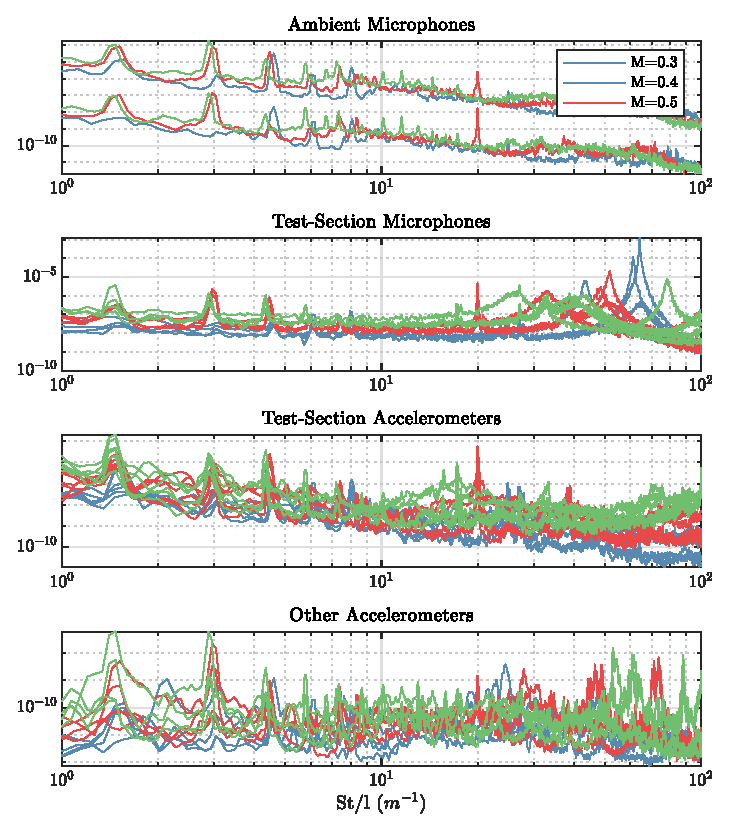
\includegraphics{../matlab/07_multiple_sensor_filtering/sensor_spectra.eps}
  \caption{Power-spectra of the additional sensor measurements at the three Mach numbers tested. The x-axis is in Strouhal number per characteristic length ($St/l$).}
  \label{fig:07_sensor_spectra}
\end{figure}
These plots are presented as Strouhal number per characteristic length with the different groups of sensors shown together.
The blade-passing frequency for these data sets is at a $St/l$ of approximately 3-$m^{-1}$ with a clear and consistant narrow-band signal at for but the $M=0.3$ run which has a slight increase in signal for some of the sensors.
For the $M=0.5$ case there is an additional strong narrow-band signal at 20-$m^{-1}$ for all sensors and a slightly broader signal at 38-$m^{-1}$ that is only present in the test-section mounted sensors that may be due to extra fan vibration which is currently limiting the top speed of the wind-tunnel.
The test-section mounted microphones are picking up boundary layer accoustic noise above $St/l$ of approximately 20-$m^{-1}$.

Two variants of this filtering technique were tried.
The first was a standard LSE-SPOD technique in which the spectral POD was performed on the data set that was Fourier transformed in time only.
The second will be referred to here as LSE-MSPOD, in which the spectral POD was applied to a data set in which the Fourier transformed was performed in all dimensions of space and time.
Figures \ref{fig:07_lse_spod} and \ref{fig:07_lse_mspod} show multi-dimensional power spectrum plots at a temporal block length of $2^{10}$ with no overlap.
\begin{figure}
  \centering
  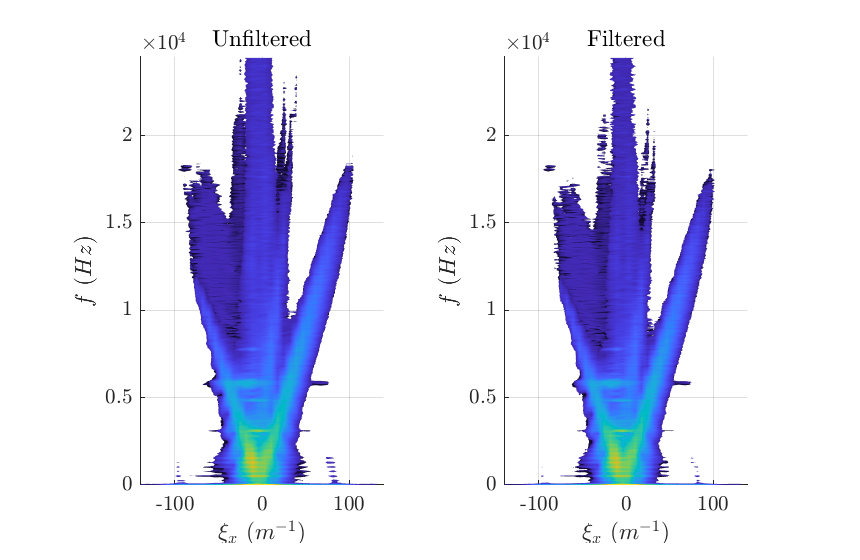
\includegraphics{../matlab/07_multiple_sensor_filtering/lse_spod.eps}
  \caption{A multi-dimensional power spectrum of an unfiltered wavefront and the same wavefront filtered with the LSE-SPOD method using all 16 additional microphone or accelerometer measurements.  }
  \label{fig:07_lse_spod}
\end{figure}
\begin{figure}
  \centering
  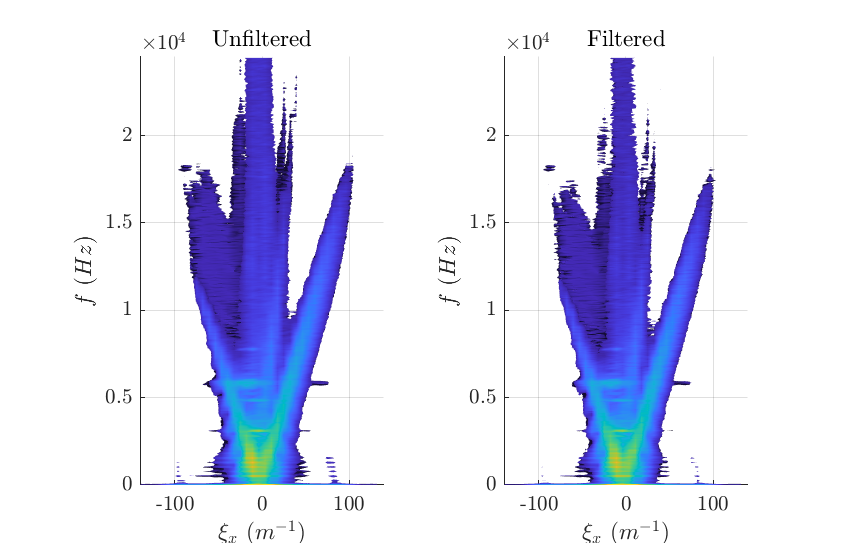
\includegraphics{../matlab/07_multiple_sensor_filtering/lse_mspod.eps}
  \caption{A multi-dimensional power spectrum of an unfiltered wavefront and the same wavefront filtered with the LSE-MSPOD method using all 16 additional microphone or accelerometer measurements.  }
  \label{fig:07_lse_mspod}
\end{figure}
These plots show a combination of the isosurface and horizontal moving plane-wave slice.
Both of these methods preformed effectively identical to one another with a drop of 14.2\% drop in overall RMS value of the filtered wavefront (both time and space).
There is a significant drop in the signal at the blade-passing frequency and its harmonics, especially at the higher spatial frequencies.
The stationary signal information is also significantly reduced along with the high temporal-frequency acoustic signal.
The aero-optical boundary layer signal is also partially reduced, which is most noticeable at higher temporal-frequencies.
Some of this lost signal can be restored by increasing the overlap of the temporal frequency blocks, but this also restores some of the unwanted high temporal-frequency contamination.

\begin{table}
  \centering
  \caption{$\opdrms$ ($\mu m$) comparison using different combinations of additional sensor information in the LSE-MSPOD filtering process.}
  \input{../matlab/07_multiple_sensor_filtering/lse_mspod_table.txt}
  \label{tab:07_lse_mspod_table}
\end{table}

Table \ref{tab:07_lse_mspod_table} shows the time averaged $\opdrms$ of three different data sets at a beam angle through the test-section of $90^\circ$.
The data sets were at Mach numbers of 0.3, 0.4 and 0.5 that had an unfiltered $\opdrms$ of 0.0561, 0.0521, and 0.0824 $\mu m$ respectively.
Note that in the raw processed wavefronts for the Mach number of 0.3 was higher than the 0.4 case.
There was a significant drop of between 62.6 and 78.6\% in the $\opdrms$ by removing the Zernike modes corresponding to tip and tilt.
It is at this point the Mach number of 0.4 case has a higher $\opdrms$ than the 0.3 case as would be expected {\color{red}{Reference an equation or source (probably a non-dimensionalization equation)}}.

Five different combinations of additional sensors were examined for filtering with the LSE-MSPOD process.
The first set was all of the accelerometers which resulted in an additional drop in $\opdrms$ of between 3 and 5\%.
The second and third sets used either the ambient or duct microphones and those sets had slightly less reduction than the accelerometers resulted in.
The forth set was the test-section sensors that was comprised of six window mounted accelerometers and four duct mounted microphones.
This set of sensors preformed the same as all of the accelerometers, while the use of all of the additional sensors in the last set performed the best, with an additional reduction in $\opdrms$ of 4 to 6\% from the tip/tilt removal cases.

A velocity filter was also tried in addition to just the tip/tilt removal or in conjunction with tip/tilt and all the sensors being used in the LSE-MSPOD process.
The velocity filter performed better than the all sensors removal case by an additional 1.5 to 3\%.
When all sensors were used with LSE-MSPOD on the velocity filtered wavefronts an additional 3 to 4\% of the $\opdrms$ was removed from just the velocity filtered case or an additional 8.1\% reduction for only doing tip/tilt removal on the Mach number of 0.3 case or 14.1 and 13.3\% reduction for the 0.4 and 0.5 Mach number cases.

Using either the temporal or multi-dimensional version of the LSE-SPOD filtering technique can help remove some of the narrow-band acoustic and vibration reduction in an optical wavefront.
This additional reduction does seem to be somewhat tied to the number of sensors used with more sensors having a greater impact on the signal reduction.
Since the vibrations and acoustics have the same primary source, the wind-tunnel fan, they seems to do a relatively equivalent job at filtering the optical contamination.
Accelerometers have a benefit easier installation but the microphones do not necessary have to be installed inside of the wind-tunnel.
